\section{Praktikos vietos aprašymas}

\subsection{Įmonės apibūdinimas}
UAB „INVENTI“ yra 2011 metais įkurta įmonė, kuri siūlo informacinių sistemų kūrimo ir integracijos paslaugas,
taikydama inovatyvius sprendimus siekiant sukurti pridėtinę vertę savo klientams.
Imonėje dirba specialistai, turintys didelę patirtį kuriant ir integruojant sudėtingas bankininkystės, veiklos optimizavimo, elektroninių paslaugų,
valstybės informacines sistemas, registrus. Didžiausią patirtį turi finansų sektoriuje.
Naudodami pažangią projektų vykdymo metodiką Agile, „INVENTI“ sumažina projekto riziką, dinamiškai reaguodama į pasikeitimus ir užtikrindama terminų laikymąsi.
Taikydama iteracinį sistemų kūrimo metodą, svarbiausius sistemos funkcionalumus gali pateikti dalimis, pagal kliento prioritetus \ref{img:clients}.

\begin{figure}[H]
    \centering
    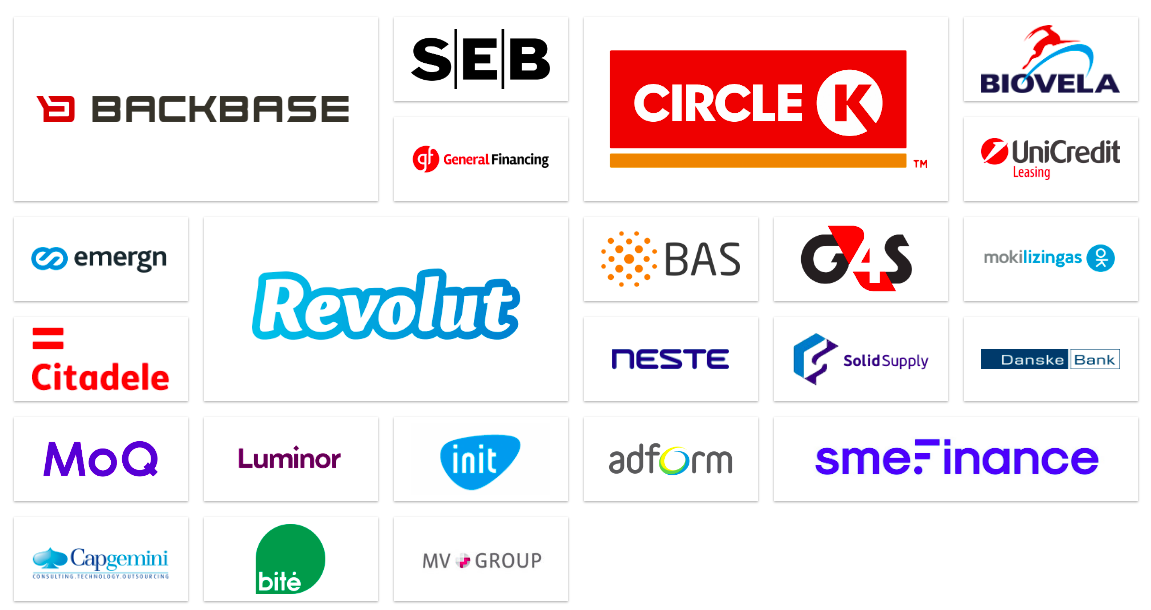
\includegraphics[scale=0.4]{img/clients.png}
    \caption{UAB „INVENTI“ įmonės klientai (paimta iš įmonės puslapio).}
    \label{img:clients}
\end{figure}


\subsection{Įmonės organizacinė struktūra}
Šiuo metu įmonėje dirba 33 darbuotojai. Kiekvienas projektas turi savo komandą,
ir komandų dydis priklauso nuo projekto apimties, prie vieno projekto dirba nuo 1 iki 10 žmonių, be projekto vadovo. Projektų vadovai vienu metu gali
vadovauti keliems projektams. Mano komandoje be projekto vadovo dirbo 4 žmonės. Įmonėje didžiausia dalis kolektyvo yra programuotojai, jiems vadovauja keli projektų vadovai,
taip pat yra devOps inžinierius, žmogiškųjų išteklių specialistė, administratorė ir direktorius.


\subsection{Darbo sąlygos}
Įmonės ofisas randasi Lvovo g. 105A, Vilnius, moderniame verslo centre „Park Town“, 3 aukšte. Darbuotojams suteikiamos parkavimo vietos, kurios randasi prie Fanų stadiono.
Peščiomis ofisą galima pasiekti per 4 minutes. „Park Town“ objektas sudarytas iš dviejų pastatų, viename iš jų yra „Lunch up“ restoranas, į kurį ofisų darbuotojai ateina pietauti.
Taip pat yra sporto salė „RE. FORMATAS“. Įmonė aprūpina visomis darbo priemonėmis, nešiojamu kompiuteriu, dviem monitoriais ir kitais įmonės identiteto atributais, pavyzdžiui,
kuprinė, marškiniai, užrašų knygelė. Taip pat naujas darbuotojas gauna magnetinę kortelę, skirta patekti į ofisą.
Ofisas yra atviros erdvės, vienoje erdvėje dirba 10-12 žmonių, visi komandos nariai sėdi vienoje erdvėje.
Ofise yra kelios erdvės pokalbiams, susitikimams. Kiekviena erdvė, arba konferencijų salė turi unikalų pavadinimą, pagal tam tikrą atributą, pavyzdžiui,
erdvė, kurioje sienos yra iš stiklo, vadinama akvariumu. Darbuotojų poilsiui įrengtas poilsio kambarys, taip pat įrengta virtuvėlė,
kurioje dažnai vyksta įvairūs renginiai, pavyzdžiui, švenčiami gimtadieniai, projektų užbaigimas, „tech-talk'ai“.

Darbo laikas nėra fiksuotas, tačiau standartiškai, darbuotojai ateina į darbą nuo 7 iki 10 ryto. Išdirbtos darbo valandos fiksuojamas „Clockify“, kur projektų vadovai veda
komandos išdirbtų valandų statistiką, pagal kurią atitinkamai išrašo klientams sąskaitas.
Pirma diena atėjęs į darbą, darbuotojas darbo vietoje randa lapelį, kuriame trumpai supažindinama su kolektyvu, nurodoma, kas kur sėdi, į ką kreiptis, kilus įvairiems klausimams.
Taip pat gauna prieigas prie „G-mail“ el. pašto ir vidinių sistemų, tokiu kaip „JIRA“, „Confluence“. Bendravimas tarp įmonės darbuotojų vyksta per „Slack“ sistemą.